/%%%%%%%%%%%%%%%%%%%%%%%%%%%%%%%%%%%%%%%%%%%%%%%%%%%%%%%%%%%%%%%%%%%%%%%%%%%%%%%%
%                                                                              %
%            A Painless Introduction to Programming UAMMD Modules              %
%                    Chapter 2: Unleash your own potential                     %
%                                                                              %
%                          Marc Meléndez Schofield                             %
%                                                                              %
%%%%%%%%%%%%%%%%%%%%%%%%%%%%%%%%%%%%%%%%%%%%%%%%%%%%%%%%%%%%%%%%%%%%%%%%%%%%%%%%

You can only have so much fun playing with a Lennard-Jones simulation. Changing
the parameter values and then looking for differences in your plots gets old
soon. If you've made it this far, you want more. You imagine molecules, or
larger structures. Perhaps you'd like to simulate billowing smoke, sloshing
water, or planets orbiting a star. All in good time.

Whatever your final aim, you need new interactions, and this chapter contains a
good collection of them.

\section{Harmonic bonds}

The simplest permanent link between particles in UAMMD has to be the harmonic
bond. Think of it as an invisible linear spring connecting two particles. As
long as they remain at the equilibrium distance $r_0$, they exert no force on
each other, but when you stretch their separation $r$, they pull back. The
potential function for this bond, then, equals
\begin{equation*}
  V(r) = \frac{1}{2}\ K\ (r - r_0)^2,
\end{equation*}
where the spring constant $K$ quantifies the bond rigidity.

Take a string of one hundred and one particles as our explanatory device. We
will line them all up along a curved queue, standing initially at rest.
\label{stringInitialConditions}
\begin{lstlisting}
%! codeblock: stringInitialConditions
  int numberOfParticles = 101;
  auto particles
    = make_shared<ParticleData>(numberOfParticles, sys);

  {
    auto position
      = particles->getPos(access::location::cpu,
                          access::mode::write);
    auto velocity
      = particles->getVel(access::location::cpu,
                          access::mode::write);

    real amplitude = 0.1;
    real stringlength = 1.0;
    int modenum = 1;
    for(int i = 0; i < numberOfParticles; ++i) {
      position[i].x = i*(stringlength/(numberOfParticles - 1));
      position[i].y = amplitude*sin(modenum*M_PI*position[i].x);
      position[i].z = position[i].w = 0;
      velocity[i].x = velocity[i].y = velocity[i].z = 0;
    }
  }
%! codeblockend
\end{lstlisting}

UAMMD reads bond information in from an external file. Let me first explain the
format of this plain text bond file. It should look something like this:
\begin{lstlisting}
100
0 1 1000.0 0.01
1 2 1000.0 0.01
2 3 1000.0 0.01
3 4 1000.0 0.01
    . . .
\end{lstlisting}
and so on. The file begins with the number of bonds ($100$) followed by a row
for each bond presenting $i$, $j$, $K$ and $r_0$, that is, the particle ID
numbers, the bond spring constant and the equilibrium distance. Hence, the next
line links particles $0$ and $1$ with a bond of $K = 1000.0$ and $r_0 = 0.01$.
After that, we get the values for the bond connecting particles $1$ and $2$.
Even though I have chosen identical values of $K$ and $r_0$ for all the bonds in
this example, you can of course make them all different if you like.

In addition to linking particles, you can attach them to fixed points in space.
We will pin particle $0$ to the origin of coordinates and particle $100$ to
point $(1, 0, 0)$. After the previous list of bonds, we must include the number
of fixed bonds (only $2$ in our case). The format for these is simply $i$, $x$,
$y$, $z$, $K$, $r_0$, meaning: particle ID, position in space $(x, y, z)$,
spring constant and equilibrium distance. So in our example, the bond file
should end with:
\begin{lstlisting}
2
0 0 0 0 1000.0 0.0
100 1 0 0 1000.0 0.0
%!
\end{lstlisting}
With the ends held in place, we have a taut string. As soon as we let go and run
the simulation, it should vibrate.

We will make the program write the bond information so that we don't have to.
\begin{lstlisting}
%! codeblock: stringBondFile
  {
    std::ofstream bondInfo("data.bonds");
    if(not bondInfo.is_open()) {
      sys->log<System::CRITICAL>("Unable to create data.bonds file. Halting program.");
      exit(-1);
    }

    bondInfo<<(numberOfParticles - 1)<<endl;
    for(int i = 0; i < numberOfParticles - 1; ++i) {
      bondInfo<<i<<" "<<(i + 1)<<" 1000.0 0.01"<<endl;
    }
    bondInfo<<"2"<<endl;
    bondInfo<<"0 0 0 0 1000.0 0.0"<<endl;
    bondInfo<<"100 1 0 0 1000.0 0.0"<<endl;
  }
%! codeblockend
\end{lstlisting}

Including the bonds presents no difficulties from the point of view of UAMMD
code, as the code resembles the lines we wrote for the Lennard-Jones
interaction. You insert the customary include at the top,
\begin{lstlisting}
# include "Interactor/BondedForces.cuh"
%!
\end{lstlisting}
define the interaction parameters to create the ``interactor'',
\begin{lstlisting}
%! codeblock: stringBondInteractor
  {
    using HarmonicBonds = BondedForces<BondedType::Harmonic>;
    HarmonicBonds::Parameters bondParameters;
    bondParameters.file = "data.bonds";
    auto bonds = make_shared<HarmonicBonds>(particles, sys, bondParameters);
%! codeblockend
\end{lstlisting}
and then add the new bond interaction to the integrator.
\begin{lstlisting}
%! codeblock: stringAddInteractor
    integrator->addInteractor(bonds);
  }
%! codeblockend
\end{lstlisting}

To replicate the simulation results shown in Figure \ref{vibratingString},
set the integrator parameters to these values:
\begin{lstlisting}
%! codeblock: VerletParameters
  using Verlet = VerletNVE;
  Verlet::Parameters VerletParams;
  VerletParams.dt = 0.001;
  VerletParams.initVelocities=false;
%! codeblockend
\end{lstlisting}
For the figure, I simulated twenty thousand steps and output the positions every
two thousand. Because I did not need a simulation box in this case, I eliminated
the corresponding block of code and changed the output command.
\begin{lstlisting}
      out<<endl;
      for(int id = 0; id < numberOfParticles; ++id)
        out<<position[index[id]]<<endl;
%!
\end{lstlisting}

\begin{comment}
Vibrating string simulation code:
\begin{lstlisting}
%! codefile: code/vibratingString.cu
# include "uammd.cuh"
# include "utils/InitialConditions.cuh"
# include "Interactor/BondedForces.cuh"
# include "Integrator/VerletNVE.cuh"

using namespace uammd;
using std::make_shared;
using std::endl;

int main(int argc, char *argv[]){

  auto sys = make_shared<System>(argc, argv);

  %! codeinsert: stringInitialConditions

  %! codeinsert: VerletParameters

  %! codeinsert: Verlet src: chapters/first_simulation.tex

  %! codeinsert: stringBondFile

  %! codeinsert: stringBondInteractor

  %! codeinsert: stringAddInteractor

  std::string outputFile = "vibratingString.dat";
  std::ofstream out(outputFile);

  int numberOfSteps = 20000;
  int printEverynSteps = 2000;

  %! codeblock: integrate
  for(int step = 0; step < numberOfSteps; ++step) {
    integrator->forwardTime();

    if(printEverynSteps > 0
       and step % printEverynSteps == 1) {
      auto position
        = particles->getPos(access::location::cpu,
                            access::mode::read);
      const int * index = particles->getIdOrderedIndices(access::location::cpu);

      out<<endl;
      for(int id = 0; id < numberOfParticles; ++id)
        out<<position[index[id]]<<endl;
    }
  }
  %! codeblockend

  sys->finish();

  return 0;
}
%! codeend
\end{lstlisting}
\end{comment}

\begin{figure}
  \centering
  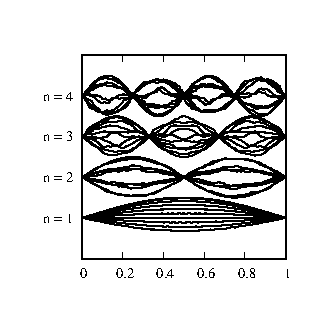
\includegraphics[width = 0.6 \textwidth]{figures/vibratingString.eps}
  \caption{\label{vibratingString}A chain of $101$ particles connected with
           harmonic bonds and ends tethered to fixed points. It (imperfectly)
           follows the behaviour of the ideal vibrating string. The first four
           normal modes of vibration were achieved by setting the
           \texttt{modenum} variable (see page
           \pageref{stringInitialConditions}) to $n = 1, 2, 3,$ and $4$.}
\end{figure}

\section{External fields}

Figure \ref{vibratingString} may hold the attention of harmonic analysis
enthusiasts but, personally, I cannot wait to free the chain of particles at one
end and simulate a swinging rope. We already know how to deal with the bonds.
Just eliminate the final fixed bond in the data.bonds file, leaving the end of
the file like this:
\begin{lstlisting}
1
0 0 0 0 1000.0 0.0
%!
\end{lstlisting}

We are holding our chain only from the side at the origin of coordinates, but if
we expect to watch it swing back and forth, we cannot forget to implement the
force driving this motion: gravity.

Surely, we can add gravity into the mix with ease, right? It cannot be worse
than the Lennard-Jones potential or harmonic bonds. Well \ldots in a sense, it
does not differ much. You can incorporate it just as you would any other
interaction. Unfortunately, UAMMD was not designed with a standard gravity
interaction in mind, so we will have to write our own. Not to worry, though. We
will find it instructive and not too difficult.

In our model, gravity will appear as an external force field, meaning that it
does not act as an interaction among particles, but rather a force field that
affects each of them independently of the motions of the other particles. Thus,
\begin{lstlisting}
# include "Interactor/ExternalForces.cuh"
%!
\end{lstlisting}

An external force definition consists of four parts:
\begin{enumerate}
  \item A setup.
  \item A rule for how to calculate the force on a particle.
  \item A rule for the particle energy due to the external field.
  \item A function that obtains the information needed to calculate the force
        and energy.
\end{enumerate}
In terms of code, we create a data structure with a real value $g$ for the
accleration of gravity.
\begin{lstlisting}
%! codeblock: gravityDefinition
struct gravitationalForce{
  real g;
%! codeinsert: gravityConstructor
%! codeinsert: gravityForce
%! codeinsert: gravityEnergy
%! codeinsert: gravityParticleInfo
};
%! codeblockend
\end{lstlisting}
Now, between the declaration of $g$ and the closing bracket, we will insert the
four items listed above, beginning with a function that initialises the force.
It should only do one thing, take the numerical value given to $g$ and assign it
to the variable \texttt{g}. We can code it as an empty function.
\begin{lstlisting}
%! codeblock: gravityConstructor
  gravitationalForce(real numericalValueOfg):g(numericalValueOfg){}
%! codeblockend
\end{lstlisting}
The second item (the force) equals the mass of the particle times $-g$ in the
$y$ direction.
\begin{lstlisting}
%! codeblock: gravityForce
  __device__ __forceinline__ real3 force(const real4 &position, const real &mass){
    return make_real3(0.0f, -mass*g, 0.0f);
  }
%! codeblockend
\end{lstlisting}
Next, we write the function for the gravitational potential energy.
\begin{lstlisting}
%! codeblock: gravityEnergy
  __device__ __forceinline__ real energy(const real4 &position, const real &mass){
    return mass*g*position.y;
  }
%! codeblockend
\end{lstlisting}
We end the data structure telling the interaction where to get the position and
mass information.
\begin{lstlisting}
%! codeblock: gravityParticleInfo
  std::tuple<const real4 *, const real *> getArrays(ParticleData *particles){
    auto position = particles->getPos(access::location::gpu, access::mode::read);
    auto mass = particles->getMass(access::location::gpu, access::mode::read);
    return std::make_tuple(position.raw(), mass.raw());
  }
%! codeblockend
\end{lstlisting}
You might have asked yourself why we handed the position over to the force
function even though it doesn't need to know the particle's location. The reason,
you might have guessed, lies in the tuple function, which extracts information
from the \texttt{particles} information and sends the same arguments to both the
force and energy functions.

Imagine we pull the rope out to the right. In addition to the positions and
velocities, we must also define the mass of each element in the rope.
\begin{lstlisting}
%! codeblock: ropeInitialConditions
  {
    auto position
      = particles->getPos(access::location::cpu,
                          access::mode::write);
    auto velocity
      = particles->getVel(access::location::cpu,
                          access::mode::write);
    auto mass
      = particles->getMass(access::location::cpu,
                          access::mode::write);

    real stringlength = real(1.0);
    for(int i = 0; i < numberOfParticles; ++i) {
      position[i].x = i*(stringlength/(numberOfParticles - 1));
      position[i].y = position[i].z = position[i].w = real(0.0);
      velocity[i].x = velocity[i].y = velocity[i].z = real(0.0);
      mass[i] = real(0.001);
    }
  }
%! codeblockend
\end{lstlisting}
It does not matter much whether you write the numerical values as \texttt{1.0}
or \texttt{real(1.0)} here. I recommend you get used to the second option in
UAMMD. It will help the compiler speed up your code by casting the floating
point number to the right precision.

To create the gravitational interaction and add it to the integrator, follow the
standard procedure.
\begin{lstlisting}
%! codeblock: gravityInteraction
  {
    auto gravity
      = make_shared<ExternalForces<gravitationalForce>>(particles, sys, make_shared<gravitationalForce>(real(9.8)));

    integrator->addInteractor(gravity);
  }
%! codeblockend
\end{lstlisting}

Time for an important warning. If you want your code to compile with the changes
in this section, you must appease the spirits of \texttt{nvcc} with the flag
\texttt{--expt-relaxed-constexpr}.
\begin{lstlisting}
nvcc -I../uammd/src -I../uammd/src/third_party --expt-relaxed-constexpr -o swingingRope swingingRope.cu
\end{lstlisting}
as well as any other relevant options on your system. When all the pieces fit
together nicely, you should be able to reproduce Figure \ref{swingingRope}.

\begin{figure}[t]
  \centering
  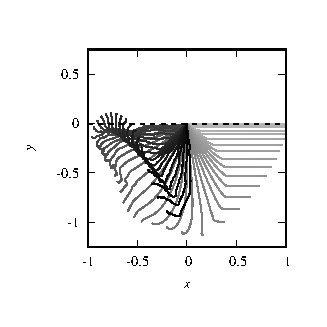
\includegraphics[width = 0.6 \textwidth]{figures/swingingRope.eps}
  \caption{\label{swingingRope}A chain of $101$ particles connected with
           harmonic bonds attached to the origin behaves like a swinging rope
           in a gravitational field. \textit{Parameters}: time step
           $dt = 10^{-4}$, 15000 steps printing every 300 steps.}
\end{figure}


\begin{comment}
Swinging rope simulation code:
\begin{lstlisting}
%! codefile: code/swingingRope.cu
# include "uammd.cuh"
# include "utils/InitialConditions.cuh"
# include "Interactor/BondedForces.cuh"
# include "Interactor/ExternalForces.cuh"
# include "Integrator/VerletNVE.cuh"

using namespace uammd;
using std::make_shared;
using std::endl;

%! codeinsert: gravityDefinition

int main(int argc, char *argv[]){

  auto sys = make_shared<System>(argc, argv);

  int numberOfParticles = 101;
  auto particles
    = make_shared<ParticleData>(numberOfParticles, sys);

  %! codeinsert: ropeInitialConditions

  using Verlet = VerletNVE;
  Verlet::Parameters VerletParams;
  VerletParams.dt = real(0.0001);
  VerletParams.initVelocities=false;

  %! codeinsert: Verlet src: chapters/first_simulation.tex

  {
    std::ofstream bondInfo("data.bonds");
    if(not bondInfo.is_open()) {
      sys->log<System::CRITICAL>("Unable to create data.bonds file. Halting program.");
      exit(-1);
    }

    bondInfo<<(numberOfParticles - 1)<<endl;
    for(int i = 0; i < numberOfParticles - 1; ++i) {
      bondInfo<<i<<" "<<(i + 1)<<" 1000.0 0.01"<<endl;
    }
    bondInfo<<"1"<<endl;
    bondInfo<<"0 0 0 0 1000.0 0.0"<<endl;
  }

  %! codeinsert: stringBondInteractor

  %! codeinsert: stringAddInteractor

  %! codeinsert: gravityInteraction

  std::string outputFile = "swingingRope.dat";
  std::ofstream out(outputFile);

  int numberOfSteps = 15000;
  int printEverynSteps = 300;

  %! codeinsert: integrate

  sys->finish();

  return 0;
}
%! codeend
\end{lstlisting}
\end{comment}

\section{Other types of bonds}

Harmonic bonds thread points together easily, but some circumstances require
other specialised types of bonds. Take a polymer strand in solution and zoom in
on a section of a few hundred monomers. It may behave like a harmonic spring
when you try to stretch it, but it will not extend indefinitely without
breaking. Harmonic potentials, in contrast, allow you to stretch a bond
indefinitely as long as you pull hard enough.

In settings like polymer research you would prefer a finitely extensible
nonlinear  elastic (FENE) bond. FENE bonds have a potential function given by
\begin{equation*}
  V_\text{FENE}(r) = -\frac{1}{2} K r_0^2\ 
                \ln\left(1 - \left(\frac{r}{r_0}\right)^2\right).
\end{equation*}
Note that the minimum value for $V_\text{FENE}(r)$ (with $r \geq 0$) lies at $r
= 0$, so the force will tend to pull the particles on top of each other.
Customarily, researchers combine FENE bonds with the repulsive part of
Lennard-Jones potentials, making the interaction potential between two bonded
particles equal to
\begin{equation*}
  V(r) =
    \begin{cases}
         V_\text{FENE}
         + \epsilon
         + 4\epsilon\left(\left(\frac{\sigma}{r}\right)^{12}
                        - \left(\frac{\sigma}{r}\right)^6\right),
         & \text{ for } r \leq \sqrt[6]{2} \sigma, \\
         V_\text{FENE}
         & \text{ for } r > \sqrt[6]{2} \sigma.
    \end{cases}
\end{equation*}
Furthermore, note that $V(r)$ diverges as $r$ approaches $r_0$. This guarantees
that particles will never separate further than $r_0$ as long as you choose
small enough integration time steps.

Within UAMMD, code for FENE bonds parallels that of harmonic bonds, but with a
different type, so you would define them with
\begin{lstlisting}
    using FENEBonds = BondedForces<BondedType::FENE>;
\end{lstlisting}
When experimenting with FENE bonds, remember that linked particles must start
off with a separation smaller than $r_0$.

A different special case arises when modelling periodic structures. Picture an
infinite chain of particles stretching across the simulation box from left to
right. This we can simulate with periodic boundary conditions, but note that we
have to connect the leftmost particle not to the last particle on the right, but
rather to its periodic image to the left. Similarly, the particle closest to the
right of the box attaches to a periodic image of the first particle on the left.
Clearly, a bond crossing the whole width of the box will not do. We must specify
that a bond between particles $i$ and $j$ means between $i$ and the closest
periodic image of $j$ and viceversa. These types of bonds were named HarmonicPBC
and FENEPBC in UAMMD.

The final part of this chapter explains how to define your own bond types, after
the following section on angular potentials.

\section{Angular potentials}

How do you transform a rope into a flexible rod in UAMMD? Probably the easiest
route simply adds more bonds. Instead of connecting particles in a line only to
their nearest neighbours, connect them also to particles lying farther away.
This approach is known as building an elastic network, and has many practical
applications.

Now imagine a molecule formed by atoms labelled $i$, $j$ and $k$, as in Figure 
\ref{angularPotential}. Bonds connect particles $i$ and $j$, and particles $j$ 
and $k$. We could get the molecule to form the right angle $\theta$ by adding in 
an extra bond between $i$ and $k$. If we wish to study the vibrations of our 
molecule, we wouldn't usually employ that approach, though. Here's why. Forces 
should tend to restore $\theta$ when the molecule undergoes a deformation that 
changes this angle, but we can stretch the bond between $i$ and $k$ without 
altering the angle $\theta$ by stretching the other two bonds in the the same 
proportion. We would cause a force between $i$ and $k$ that should not be there. 
Contrariwise, you can devise configurations with angles different from $\theta$ 
while keeping the bond between $i$ and $k$ at the equilibrium length, achieving 
a configuration where there is no force between $i$ and $k$ even though there 
should be one. As a result, you get a molecule that doesn't wobble as it should.

\begin{figure}
  \centering
  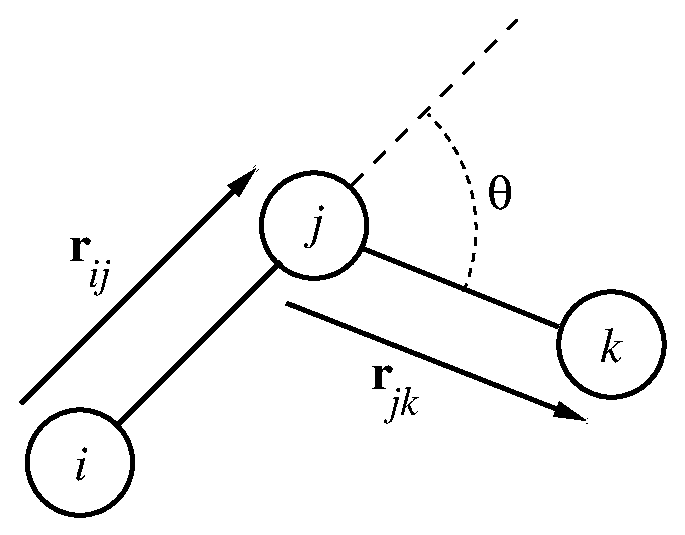
\includegraphics[width = 0.5 \textwidth]{figures/angularSprings.eps}
  \caption{\label{angularPotential}Angular potential}
\end{figure}

We set angular potentials indicating the labels of the three particles involved,
$i$, $j$ and $k$, the rigidity $K$ and the equilibrium angle $\theta_0$. When
the particles form an angle $\theta \neq \theta_0$, they feel a force that tends
to restore $\theta$ back to $\theta_0$. The angular potentials file would start
with the number of triplets on the first line, followed by rows in which you
specify $i$, $j$, $k$, $K$ and $\theta_0$, in that order. So a file with two
angular potentials could look like this
\begin{lstlisting}
2
0 1 2 100 0
5 6 7 100 1.5708
%!
\end{lstlisting}
The first three particles would tend to lie on a straight line, while particles 
$5$, $6$ and $7$ would form a right angle. Note that $\theta_0$ refers to the 
equilibrium angle between $\mathbf{r}_{ij}$ and $\mathbf{r}_{jk}$ (see Fig. 
\ref{angularPotential}).

With the sole intention of showing you how angular potentials work, we'll 
transform our rope in the previous code into something like a fiberglass cable, 
in that it opposes bending slightly.

For starters, we hold the inital tenth of the cable horizontally with
fixed-point bonds, and let gravity bend the rest of the cable.
\begin{lstlisting}
%! codeblock: cableFixedBonds
    bondInfo<<"10"<<endl;

    real beamlength = real(1.0);
    for(int i = 0; i < 10; i++)
      bondInfo<<i<<" "<<i*(beamlength/(numberOfParticles - 1))<<" 0 0 1000.0 0.0"<<endl;
%! codeblockend
\end{lstlisting}
We will need a smaller time step to resolve the motion.
\begin{lstlisting}
%! codeblock: cableTimeStep
  VerletParams.dt = real(0.00001);
%! codeblockend
\end{lstlisting}
Consequently, we increase the number of steps to integrate.
\begin{lstlisting}
%! codeblock: cableNumberOfSteps
  int numberOfSteps = 150000;
  int printEverynSteps = 5000;
%! codeblockend
\end{lstlisting}

Now let us link our chain with angular potentials, by attaching every three
consecutive particles with $K = 2.0$ and $\theta_0 = 0$.
\begin{lstlisting}
%! codeblock: angularForcesFile
  {
    std::ofstream angularInfo("data.angularForces");
    if(not angularInfo.is_open()) {
      sys->log<System::CRITICAL>("Unable to create data.angularForces file. Halting program.");
      exit(-1);
    }

    real K = 2.0, theta0 = 0.0;
    angularInfo<<(numberOfParticles - 2)<<endl;
    for(int i = 0; i < numberOfParticles - 2; ++i) {
      angularInfo<<i<<" "<<(i + 1)<<" "<<(i + 2)<<" "<<K<<" "<<theta0<<endl;
    }
  }
%! codeblockend
\end{lstlisting}

If we link our UAMMD module to the relevant header,
\begin{lstlisting}
# include "Interactor/AngularBondedForces.cuh"
%!
\end{lstlisting}
creating the interaction follows the usual rules, but notice that you need to
have a simulation box defined (as explained in section \ref{simulation_box}). We
will just make the box infinite in every direction.
\begin{lstlisting}
%! codeblock: cableBox
  real L = std::numeric_limits<real>::infinity();
  Box box(make_real3(L, L, L));
%! codeblockend
\end{lstlisting}
To generate the angular forces interaction, we write code that parallels the
creation of harmonic bonds.
\begin{lstlisting}
%! codeblock: angularForces
  {
    using angularPotentials = AngularBondedForces<AngularBondedForces_ns::AngularBond>;
    angularPotentials::Parameters angularParameters;
    angularParameters.readFile = "data.angularForces";
    auto angularForces
      = make_shared<angularPotentials>(particles, sys,
                                       angularParameters,
                                       std::make_shared<AngularBondedForces_ns::AngularBond>(box));
    integrator->addInteractor(angularForces);
  }
%! codeblockend
\end{lstlisting}
I should briefly comment on three annoying peculiarities in the code snippet
above. One, the bond type has an irritatingly redundant long name:
\begin{verbatim}
AngularBondedForces_ns::AngularBond
\end{verbatim}
Two, the file name parameter in this case was set to ``\texttt{readFile}'', 
instead of ``\texttt{file}'' as it was called for harmonic bonds. Three, for 
obscure design reasons that we do not care about now, the interactor takes a 
shared pointer to the bond type as an extra parameter.

\begin{comment}
The structure of the UAMMD module code for a flexible cable follows.
\begin{lstlisting}
%! codefile: code/cable.cu
# include "uammd.cuh"
# include "utils/InitialConditions.cuh"
# include "Interactor/BondedForces.cuh"
# include "Interactor/AngularBondedForces.cuh"
# include "Interactor/ExternalForces.cuh"
# include "Integrator/VerletNVE.cuh"

using namespace uammd;
using std::make_shared;
using std::endl;

%! codeinsert: gravityDefinition

int main(int argc, char *argv[]){

  auto sys = make_shared<System>(argc, argv);

  int numberOfParticles = 101;
  auto particles
    = make_shared<ParticleData>(numberOfParticles, sys);

  %! codeinsert: ropeInitialConditions

  %! codeinsert: cableBox

  using Verlet = VerletNVE;
  Verlet::Parameters VerletParams;
  %! codeinsert: cableTimeStep
  VerletParams.initVelocities=false;

  %! codeinsert: Verlet src: chapters/first_simulation.tex

  {
    std::ofstream bondInfo("data.bonds");
    if(not bondInfo.is_open()) {
      sys->log<System::CRITICAL>("Unable to create data.bonds file. Halting program.");
      exit(-1);
    }

    bondInfo<<(numberOfParticles - 1)<<endl;
    for(int i = 0; i < numberOfParticles - 1; ++i) {
      bondInfo<<i<<" "<<(i + 1)<<" 1000.0 0.01"<<endl;
    }
    %! codeinsert: cableFixedBonds
  }

  %! codeinsert: angularForcesFile

  %! codeinsert: stringBondInteractor

  %! codeinsert: stringAddInteractor

  %! codeinsert: angularForces

  %! codeinsert: gravityInteraction

  std::string outputFile = "cable.dat";
  std::ofstream out(outputFile);

  %! codeinsert: cableNumberOfSteps

  %! codeinsert: integrate

  sys->finish();

  return 0;
}
%! codeend
\end{lstlisting}
\end{comment}

Figure \ref{cable} shows the result of running the cable program. When compared
to Figure \ref{swingingRope}, you can clearly see we have increased our chain's
aversion to bending.

\begin{figure}
  \centering
  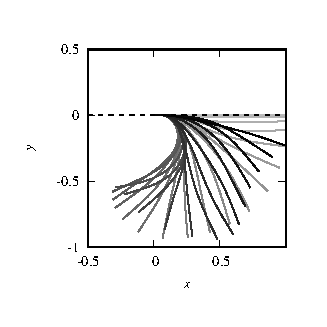
\includegraphics[width = 0.6 \textwidth]{figures/cable.eps}
  \caption{\label{cable}101 particles simulating a flexible cable bending under 
           its own weight. The leftmost tenth of the cable was held in place 
           with fixed-point bonds.}
\end{figure}


\begin{figure}
  \centering
  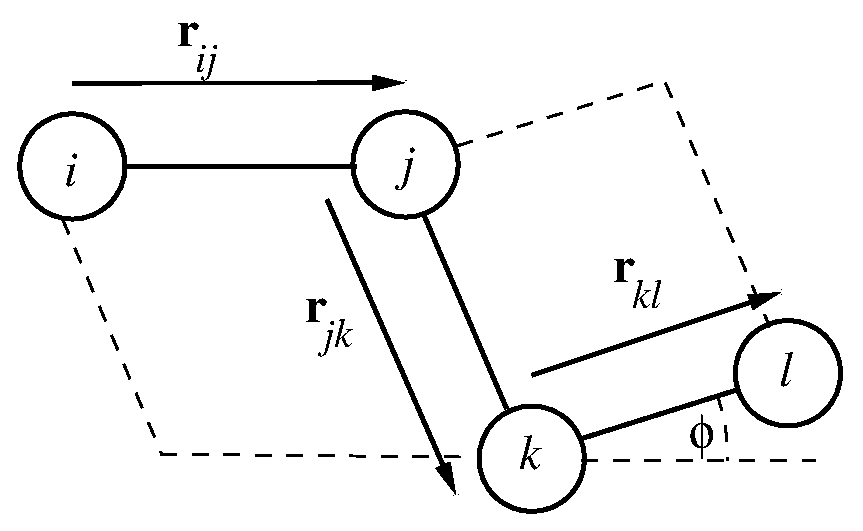
\includegraphics[width = 0.6 \textwidth]{figures/torsionalSprings.eps}
  \caption{\label{torsionalBonds}Torsional bonds}
\end{figure}

It will not surprise you to learn that the file format for these potentials
begins with the number of quartets followed by rows of $i$, $j$, $k$, $l$, $K$
and $\phi_0$ for each relevant torsion angle.

\section{Classical orbits}

\section{Defining your own potentials}

Bond potentials

Pair interactions

\begin{comment}
List of programs written in this chapter:
%! codeblock: codelist
* `vibratingString.cu`: A chain of particles linked by harmonic springs and held
   tight at the ends behaving like a vibrating string.
* `swingingRope.cu`: A chain of particles simulating a rope hanging from one of
   its ends, swinging back and forth in a gravitational field.
* `cable.cu`: A chain of particles simulating a flexible cable bending under its
   own weight.
%! codeblockend
\end{comment}
